\section{A Simple Tree Pattern}\label{sec:arb-trees}

The repository of ontology design patterns on ontologydesignpatterns.org does not contain any pattern for trees. There is also none for graphs which could have been used to specialize a trees pattern. The repository contains a pattern for lists, though,\footnote{\url{http://ontologydesignpatterns.org/wiki/Submissions:List}} and a list pattern could be generalizable to a tree pattern. 

The schema diagram for this list pattern is depicted in Figure~\ref{fig:list}. It reuses the sequence pattern\footnote{\url{http://ontologydesignpatterns.org/wiki/Submissions:Sequence}} which seems to be the relevant part for our purposes. We depict the sequence pattern schema diagram in Figure \ref{fig:sequence} and all non-tautological axioms are given in Figure \ref{fig:sequenceAxioms}.\footnote{Generated with the OWLAPI \LaTeX{} renderer \cite{eswc17-latex}.} The axiomatization appears to be rather minimalistic, e.g., ``follows'' should be transitive over ``directlyFollows'', and for a sequence we should also use cardinality restrictions to limit the number of followers and predecessors. We will return to this later on.

\begin{figure}[t]
\begin{center}
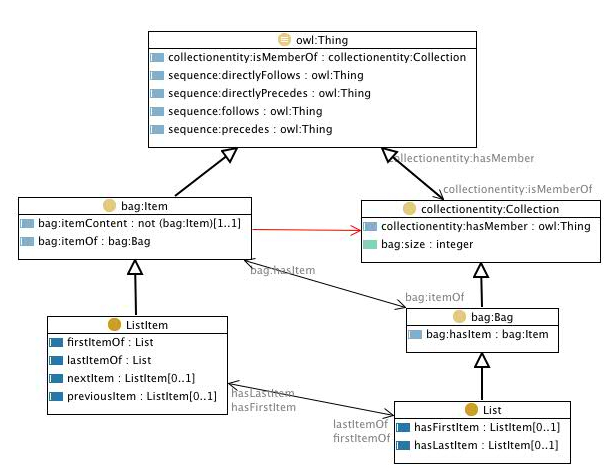
\includegraphics[width=\textwidth]{list.jpg}
\end{center}
\caption{List pattern schema diagram from ontologydesignpatterns.org}\label{fig:list}
\end{figure}

\begin{figure}[t]
\begin{center}
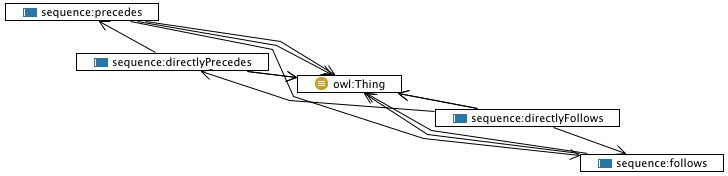
\includegraphics[width=\textwidth]{sequence.png}
\end{center}
\caption{Sequence pattern schema diagram from ontologydesignpatterns.org}\label{fig:sequence}
\end{figure}

\begin{figure}[t]
\begin{align*}
\text{directlyFollows} &\sqsubseteq  \text{follows}\\
\text{directlyFollows} &\equiv  \text{directlyPrecedes}^- \\
\text{directlyPrecedes} &\sqsubseteq  \text{precedes}\\
\text{precedes} &\equiv  \text{follows}^- \\
\text{TransitiveProperty}&(\text{follows})\\
\text{TransitiveProperty}&(\text{precedes})\\
\end{align*}
\caption{Axioms for the sequence pattern from Figure \ref{fig:sequence}. We omitted axioms that were tautologies.}\label{fig:sequenceAxioms}
\end{figure}

The list pattern just cited provides basic building blocks for a simple tree pattern. However, we opt to change the names of the properties: It seems to be more appropriate to use ``hasChild'' and ``hasDescendant'' rather than ``directlyPrecedes'' and ``precedes'', and to use ``hasParent'' and ``hasAncestor'' rather than ``directlyFollows'' and ``follows.''

Before proceeding with the tree pattern, we present a set of competency questions \cite{chess-odp-book} which seem representative to us and include operationes raised as important in Section \ref{sec:trees-of-life}:
\begin{enumerate}
\item\label{cq1} Determine the root.
\item\label{cq2}  Determine all ancestors of a given node.
\item\label{cq3}  Determine all leaves.
\item\label{cq4}  Determine all descendants of a given node.
\item\label{cq5}  Determine all descendants of a given node which are leaves.
\item\label{cq6}  Given two nodes, determine whether one is a descendant of the other. 
\item\label{cq7} Given two nodes, determine all commmon ancestors.
\item\label{cq8}  Given two nodes, determine the latest common ancestor.
\item\label{cq9}  Given two nodes $x$ and $y$, determine the earliest ancestor of $x$ which is not an ancestor of $y$.
\end{enumerate}

We next give our proposal for a simple tree pattern. Afterwards we will discuss our design choices. The schema diagram is given in Figure \ref{fig:tree}. However, the axiomatization is really much more important; it can be found in Figure \ref{fig:tree-axioms}. Note that some additional desired axioms, such as $\text{hasParent} \sqsubseteq \text{hasAncestor}$ and transitivity of hasAncestor can be inferred from the ones stated.

\begin{figure}[t]
\begin{center}
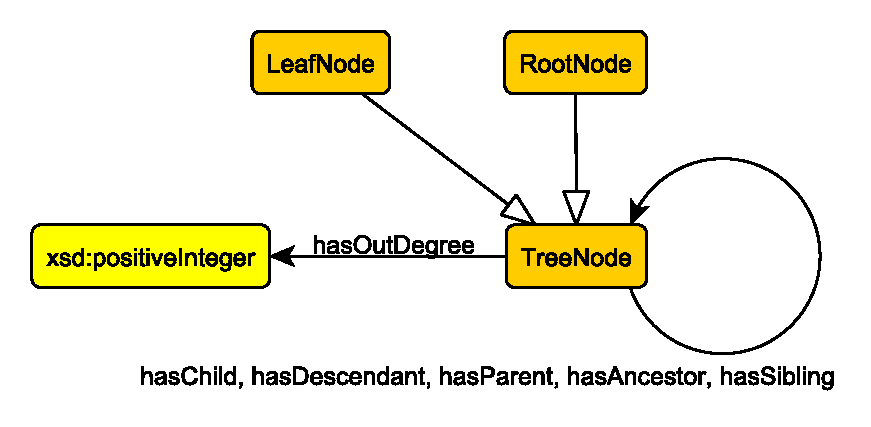
\includegraphics[width=.6\textwidth]{tree-schema}
\end{center}
\caption{Schema diagram for the simple tree pattern. Unlabelled arrows are subclass relationships.}\label{fig:tree}
\end{figure}

\begin{figure}[t]
\begin{align*}
\text{RootNode}&(a) &
\text{LeafNode}&(d) &
\text{LeafNode}&(e) \\
\text{LeafNode}&(f)&
\text{TreeNode}&(b) &
\text{TreeNode}&(c)\\
\text{hasChild}&(a,b) &
\text{hasChild}&(a,c) &
\text{hasChild}&(b,d) \\
\text{hasChild}&(b,e)&
\text{hasChild}&(c,f) &
\text{hasSibling}&(b,c)\\ 
\text{hasSibling}&(d,e) &
\text{hasOutDegree}&(a,2) &
\text{hasOutDegree}&(b,2)\\
\text{hasOutDegree}&(c,1) &
\text{hasOutDegree}&(d,0) &
\text{hasOutDegree}&(e,0)\\
\text{hasOutDegree}&(f,0)
\end{align*}
\caption{Example ABox for a tree.}\label{fig:tree-example}
\end{figure}

\begin{figure}[t]\small
\begin{align}
\text{LeafNode} &\sqsubseteq \text{TreeNode}\label{ax1}\\
\text{RootNode} &\sqsubseteq \text{TreeNode}\\
\text{TreeNode} &\sqsubseteq \forall\text{hasOutDegree}.\text{xsd:positiveInteger}\\
\text{TreeNode} &\sqsubseteq \mathord{=}1\text{hasOutDegree}.\text{xsd:positiveInteger}\\
\text{LeafNode} &\equiv \text{TreeNode} \sqcap \phantom{x}\notag\\ &\phantom{\equiv} \quad\forall\text{hasOutDegree}.\{0^{\wedge\wedge}\text{xsd:positiveInteger}\}\\
\text{TreeNode} \sqcap \neg\text{LeafNode} &\equiv \text{TreeNode} \sqcap \phantom{x} \notag\\ &\phantom{\equiv}\quad\forall\text{hasOutDegree}.\{x^{\wedge\wedge}\text{xsd:positiveInteger}\mid 1\leq x\}\label{ax6}\\
\text{hasChild} &\equiv \text{hasParent}^-\\
\text{hasDescendant} &\equiv \text{hasAncestor}^-\\
\text{hasChild} &\sqsubseteq \text{hasDescendant}\\
\text{hasDescendant} \circ \text{hasDescendant} &\sqsubseteq \text{hasDescendant}\\
\text{TreeNode} &\sqsubseteq \forall\text{hasChild}.\text{TreeNode}\\
\text{TreeNode} \sqcap \neg \text{LeafNode} &\equiv \text{TreeNode} \sqcap \exists \text{hasChild}.\text{TreeNode}\\
\text{TreeNode} &\sqsubseteq \forall\text{hasDescendant}.\text{TreeNode}\\
\text{TreeNode} &\sqsubseteq \forall\text{hasParent}.\text{TreeNode}\\
\text{TreeNode} &\sqsubseteq \forall\text{hasSibling}.\text{TreeNode}\\
\text{TreeNode} \sqcap \neg \text{RootNode} &\equiv \text{TreeNode} \sqcap \mathord{=} 1\text{hasParent}.\top\\
\text{TreeNode} &\sqsubseteq \forall\text{hasAncestor}.\text{TreeNode}\\
\text{RootNode} &\equiv \text{TreeNode} \sqcap \neg \exists\text{hasParent}.\top\\
\text{LeafNode} &\equiv \text{TreeNode} \sqcap \neg \exists\text{hasChild}.\top\\
\text{Irreflexive}&(\text{hasChild})\\
\text{Irreflexive}&(\text{hasParent})\\
\text{Irreflexive}&(\text{hasDescendant})\label{ax25}\\
\text{Irreflexive}&(\text{hasAncestor})\label{ax26}\\
\text{hasSibling} &\equiv \text{hasSibling}^-\\
\text{Irreflexive}&(\text{hasSibling})
\end{align}
\caption{Axioms for the tree pattern from Figure \ref{fig:tree}.}\label{fig:tree-axioms}
\label{figure:tree}
\end{figure}

Before we proceed, let us first make a concrete example how this pattern informs the graph structure of the ABox. Given a tree such as 
$$
\xymatrix{
& & a \ar[dl] \ar[dr] & &\\
& b \ar[dl] \ar[dr] & & c \ar[dr]&\\
d & & e & & f
}
$$
we encode it using the ABox from Figure \ref{fig:tree-example}; note that we omit redundant statements which can be inferred from the axioms. 

The axioms from Figure \ref{fig:tree-axioms} should be self-explanatory. Axiom (\ref{ax6}) uses a datatype facet. The complete set of axioms is not in OWL DL because axioms (\ref{ax25}) and (\ref{ax26}) declare irreflexivity for non-simple roles. If it is desireable to stay within OWL DL, these axioms could be omitted.

Our pattern and axiomatization include some terms which may appear to be redundant. Indeed, we could have omitted the use of hasParent and hasAncestor as these are simply inverses of hasChild and hasDescendant, respectively. Other aspects, however, are not redundant.

The property hasOutDegree may appear to be redundant, as it captures the number of children of a node. However, it is not redundant as far as the OWL model is concerned, because the underlying open world assumption makes it impossible to count the number of children. This could of course be addressed using a (local) closed world extension of OWL, such as in \cite{CarralJH12}, however the current standard does not support this. For the same reason, membership in the classes RootNode and LeafNode cannot be inferred.


\afterpage{\FloatBarrier}

The case of the hasSibling property is more intricate. Again it would naively appear as if it were redundant. However, we have not been able yet to axiomatize it in the general case; for special cases where it is possible see Section \ref{sec:bin-trees}. A naive attempt by means of a rule\footnote{This rule can be converted into OWL DL using rolification, see \cite{KrisnadhiMH11}.} 
$$\text{hasParent}(x,y) \wedge \text{hasChild}(y,z) \to \text{hasSibling}(x,z)$$ 
is insufficient because for addressing some competency questions we require irreflexivity of hasSibling, while the rule above renders hasSibling to be non-simple, which is not allowed together with irreflexivity in OWL DL.

Let us return to the competency questions listed earlier; it turns out we can address them all even when omitting the irreflexivity axioms for hasDescendant and hasAncestor, such that our model stays within OWL DL. Questions \ref{cq1} and \ref{cq3} can be addressed using the RootNode and LeafNode classes. Questions \ref{cq2} and \ref{cq4} are straightforward, as is question \ref{cq5} using the LeafNode class. Question \ref{cq6} can be solved with two queries using the hasDescendant property. 

The remaining questions are more intricate. Given two nodes $x$ and $y$, Question \ref{cq7} can be addressed via
$$\exists\text{hasDescendant}.\{x\} \sqcap \exists\text{hasDescendant}.\{y\}.$$
Question \ref{cq8} seems to require use of the hasSibling property. For readability we first give the solution as first-order predicate logic formula: 
\begin{align*}
&\phantom{\wedge} \text{hasChild}(z,w) \wedge (w=x \vee \text{hasDescendant}(w,x))\\ &\wedge \text{hasSibling}(w,v) \wedge (v=y \vee \text{hasDescendant}(v,y)).
\end{align*}
Conversion of this into OWL following the approach laid out in \cite{KrisnadhiMH11} results in the class description 
\begin{align*}
\exists\text{hasChild}.(&(\{x\}\sqcup\exists\text{hasDescendant}.\{x\})\\
&\sqcap (\exists\text{hasSibling}.(\{y\}\sqcup\exists\text{hasDescendant}.\{y\})).
\end{align*}

In a similar fashion, Question \ref{cq9} can be addressed using the class description 
$$(\{x\}\sqcup\exists\text{hasDescendant}.\{x\})\sqcap (\exists\text{hasSibling}.(\{y\}\sqcup\exists\text{hasDescendant}.\{y\})).$$

Note that irreflexivity of hasSibling is required for the class descriptions just given. Or to be more precise, what is required is that there is no node $z$ in the tree for which $\text{hasSibling}(z,z)$ is declared or can be inferred; note that this is in fact a weaker requirement than what we get by declaring irreflexivity. As a consequence, the irreflexivity declaration for hasSibling can actually be omitted from the axiomatization without impact on the just given solution to Question~\ref{cq9}; however we prefer to keep the irreflexivity declaration in the axiomatization as it disambiguates the model \cite{HitzlerK16}.   As mentioned earlier, we have not been able to find a solution to infer the (irreflexive) hasSibling relationship in the general case using OWL axioms, thus we require it as a primitive. We will revisit this in the next section, though.

Let us finally use our tree pattern to recover a list pattern based on it. The schema diagram can be found in Figure \ref{fig:list-new}. We keep only one property, hasNext, which corresponds to hasChild, and hasSuccessor, which corresponds to hasDescendant. The root becomes the first list item, the leaves become the last list item. The outdegree is always 1 unless it's the last list item, so we also omit this information. The corresponding axiomatization, as derived from the tree axiomatization above, can be found in Figure \ref{fig:list-axioms-new}. As before, Axiom (\ref{ax-list-irreflexive}) causes the pattern to fall outside OWL DL, and if this is undesirable, this axiom should be omitted.

\begin{figure}[t]
\begin{center}
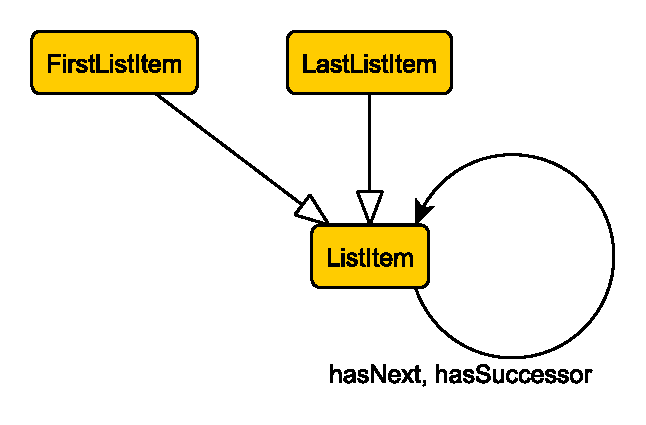
\includegraphics[width=.4\textwidth]{list-schema-new}
\end{center}
\caption{Schema diagram for the simple list pattern, derived from the tree pattern. }\label{fig:list-new}
\end{figure}

\begin{figure}[t]\small
\begin{align}
\text{FirstListItem} &\sqsubseteq \text{ListItem}\\
\text{LastListItem} &\sqsubseteq \text{ListItem}\\
\text{ListItem} &\sqsubseteq \forall\text{hasNext}.\text{ListItem}\\
\text{ListItem} &\sqsubseteq \forall\text{hasNext}^-.\text{ListItem}\\
\text{ListItem} \sqcap \neg \text{LastListItem} &\equiv \text{ListItem} \sqcap \mathord{=}1\text{hasNext}.\text{ListItem}\\
\text{ListItem} \sqcap \neg \text{FirstListItem} &\equiv \text{ListItem} \sqcap \mathord{=}1\text{hasNext}^-.\text{ListItem}\\
\text{FirstListItem} &\equiv \text{ListItem} \sqcap \neg \exists\text{hasNext}^-.\top\\
\text{LastListItem} &\equiv \text{ListItem} \sqcap \neg \exists\text{hasNext}.\top\\ 
\text{hasNext} &\sqsubseteq \text{hasSuccessor}\\
\text{hasNext} \circ \text{hasSuccessor} &\sqsubseteq \text{hasSuccessor}\\
\text{Irreflexive}&(\text{hasSuccessor})\label{ax-list-irreflexive}
\end{align}
\caption{Axioms for the lists pattern from Figure \ref{fig:list-new}.}\label{fig:list-axioms-new}
\end{figure}
